\documentclass[varwidth,border=7mm]{standalone}
\usepackage{tikz}
\usetikzlibrary{decorations.pathreplacing}
\tikzset{
  int/.style={
    decoration={brace,mirror,raise=5pt},
    postaction={decorate,draw,blue,-},
  },
  intname/.style = {pos=.5,below=8pt,blue,inner sep=1pt},
  pt/.style={above=3pt}
}
\begin{document}
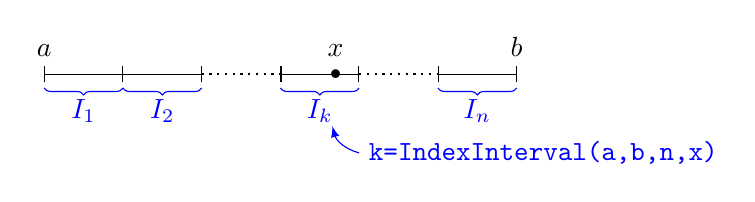
\begin{tikzpicture}
\draw[int,|-|] (0,0) node[pt]{$a$}-- +(1,0) node[intname]{$I_1$};
\draw[int,-|] (1,0) -- +(1,0) node[intname]{$I_2$};
\draw[dotted, thick] (2,0) -- +(1,0);
\draw[int,|-|] (3,0) -- +(1,0) node[intname](Ik){$I_k$} node[pos=.7,pt]{$x$} node[pos=.7,scale=3]{.};
\draw[dotted, thick] (4,0) -- +(1,0);
\draw[int,|-|] (5,0) -- +(1,0) node[intname]{$I_n$} node[pt]{$b$};
\node[right,blue,font=\tt](II) at (4,-1){k=IndexInterval(a,b,n,x)};
\draw[blue,-latex] (II.west) to[bend left] (Ik.310);

\end{tikzpicture}
\end{document}
